% begin module volumes-washer
\begin{frame}
\begin{example}[Washer Method]
\begin{columns}[c]
\column{.35\textwidth}
\psset{xunit=1cm, yunit=1cm}
\begin{pspicture}(-1,-1)(1,1)
\tiny%
\fcBoundingBox{-1.6}{-2.5}{2}{2.5}
\newcommand{\theFunOuter}{u u mul 1 add\space}%
\newcommand{\theFunInner}{u \space}%
\newcommand{\theSurface}{%
\fcSurfaceInScene[iterationsU=3, arrows=none ]{0}{0}{1}{30 \fcIterationsV\space mul}{[u v cos \theFunOuter mul v sin \theFunOuter mul]}{}%
\fcSurfaceInScene[iterationsU=3, arrows=none, colorUV={0.7 0.2 0.2}, colorVU={1 0.5 0.5} ]{0.01 }{0 }{1 }{30 \fcIterationsV  \space mul}{[u v cos \theFunInner mul v sin \theFunInner mul]}{}%
\fcSurfaceInScene[iterationsU=1, arrows=none, colorUV={1 0.5 0.5}, colorVU={0.7 0.2 0.2} ]{1 }{0 }{2 }{30 \fcIterationsV\space mul}{[1 v cos u mul v sin u mul]}{}%
}%
\renewcommand{\fcScreenStyle}{x}%
\renewcommand{\fcScreen}{[0 0 -1] 0}%
\renewcommand{\fcIterationsU}{4}%
\only<handout:2|7->{\renewcommand{\fcScreen}{[-0.05 -0.05 -1] 0}}%
\only<handout:2|8->{\renewcommand{\fcScreen}{[-0.1 -0.1 -1] 0}}%
\only<handout:2|9->{\renewcommand{\fcScreen}{[-0.15 -0.15 -1] 0}}%
\only<handout:2|10->{\renewcommand{\fcScreen}{[-0.2 -0.2 -1] 0}}%
\only<handout:2-|11->{\renewcommand{\fcScreen}{[-0.25 -0.25 -1] 0}}%
\only<handout:1|6-11>{%
\pscustom*[linecolor=\fcColorAreaUnderGraph]{%
\fcCurveIIId{0}{1}{[t t t mul 1 add 0 ]}%
\fcLineIIId[linecolor=\fcColorGraph]{[1 2 0]}{[1 1 0]}%
\fcLineIIId[linecolor=\fcColorGraph]{[1 1 0]}{[0 0 0]}%
\fcLineIIId[linecolor=\fcColorGraph]{[0 0 0]}{[0 1 0]}%
}%
}%
\fcStartIIIdScene%
\only<handout:3|16-26>{%
\fcSurfaceInScene[iterationsU=1, arrows=none, colorUV=cyan, colorVU=cyan, linecolor=cyan]{1 dict begin /u 2 3 div def \theFunInner end}{0 }{1 dict begin /u 2 3 div def \theFunOuter end}{360}{[2 3 div v cos u mul v sin u mul]}{}%
}%
\only<handout:3|15-26>{%
\fcCurveIIIdInScene[linewidth=1.5, linecolor=blue]{0}{360 }{[1 dict begin /u 2 3 div def u t cos \theFunInner 0.04 sub mul t sin \theFunInner 0.04 sub mul end]}%
\fcCurveIIIdInScene[linewidth=1.5, linecolor=blue]{0}{360 }{[1 dict begin /u 2 3 div def u t cos \theFunOuter mul t sin \theFunOuter mul end]}%
}%
\only<handout:2-|7->{\fcPutIIId{[-0.1 -0.1 1.6]}{$z$}}%
\only<7->{\fcPutIIId[lb]{[0.5 2.2 0]}{$y=x^2+1$}}%
\fcAxesIIIdFullInScene[linewidth=1, linecolor=black, arrows=->, xLabel={$x$}, yLabel={$y$},zLabel={} ]{-0.5}{-2.5}{-2.5}{1.8}{2.5}{2.5}%
\only<handout:0|12>{%
\renewcommand{\fcIterationsV}{4}%
\theSurface%
}%
\only<handout:0|13>{%
\renewcommand{\fcIterationsV}{8}%
\theSurface%
}%
\only<handout:2|14,15,27->{%
\renewcommand{\fcIterationsV}{12}%
\theSurface%
}%
\only<handout:1,2|6->{%
\fcCurveIIIdInScene[linewidth=1.5, arrows=(none), linecolor=\fcColorGraph, linewidth=1]{0}{1}{[t t t mul 1 add 0 ]}%
\fcLineIIIdInScene[linewidth=1.5, arrows=(none), linecolor=\fcColorGraph, linewidth=1]{[0 0 0]}{[1 1 0]}%
\fcLineIIIdInScene[linewidth=1.5, arrows=(none), linecolor=\fcColorGraph, linewidth=1]{[0 0 0]}{[0 1 0]}%
\fcLineIIIdInScene[linewidth=1.5, arrows=(none), linecolor=\fcColorGraph, linewidth=1]{[1 1 0]}{[1 2 0]}%
}%
\fcFinishIIIdScene%
\only<handout:0|2-5>{\fcCurveIIId[linecolor=\fcColorGraph]{-0.4}{1.2}{[t t t mul 1 add 0 ]}}%
\only<handout:0|3-5>{\fcLineIIId[linecolor=\fcColorGraph]{[-1 -1 0]}{[1 1 0]}}%
\only<handout:0|4-5>{\fcLineIIId[linecolor=\fcColorGraph]{[0 -1.6 0]}{[0 1.6 0]}}%
\only<handout:0|5>{\fcLineIIId[linecolor=\fcColorGraph]{[1 -1.6 0]}{[1 2.2 0]}}%
\only<handout:3-|28->{%
\fcLineIIId[linecolor=blue, linewidth=2pt]{[0 0 0]}{[1 0 0]}%
\fcDotIIId[linecolor=blue]{[0 0 0]}%
\fcDotIIId[linecolor=blue]{[1 0 0]}%
}%
\end{pspicture}

%\only<handout:0| 1>{%
%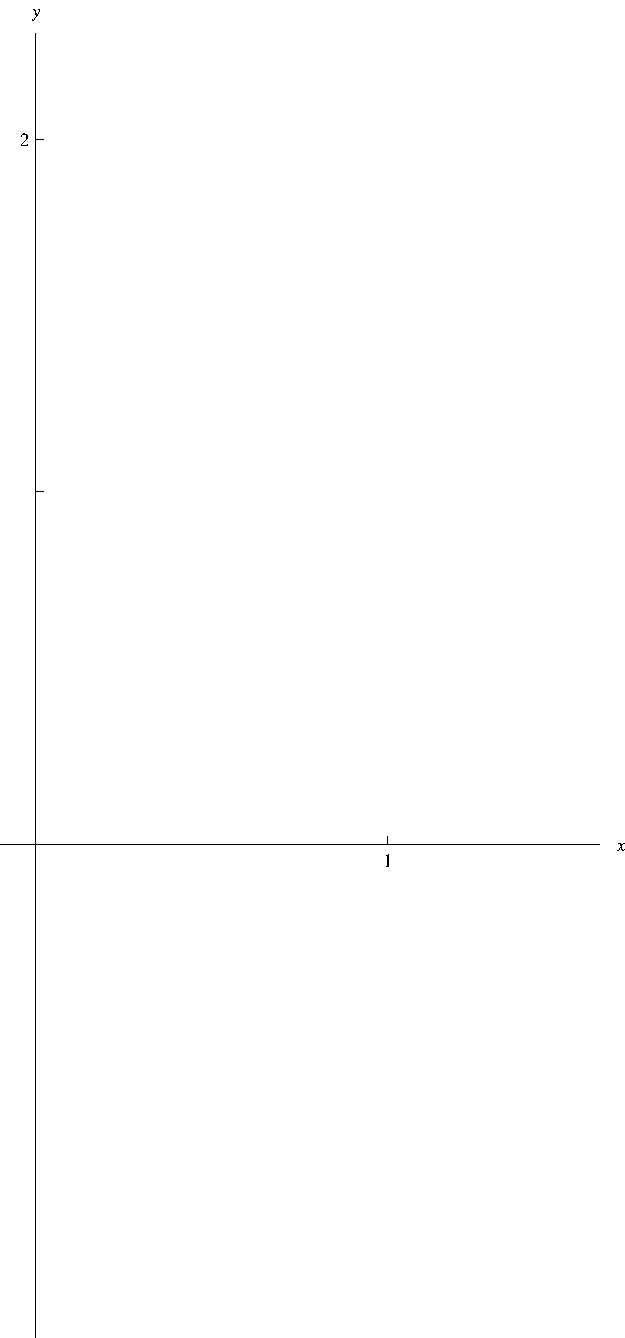
\includegraphics[height=3.3cm]{volumes/pictures/06-02-washera.pdf} %
%}%
%\only<handout:0| 2>{%
%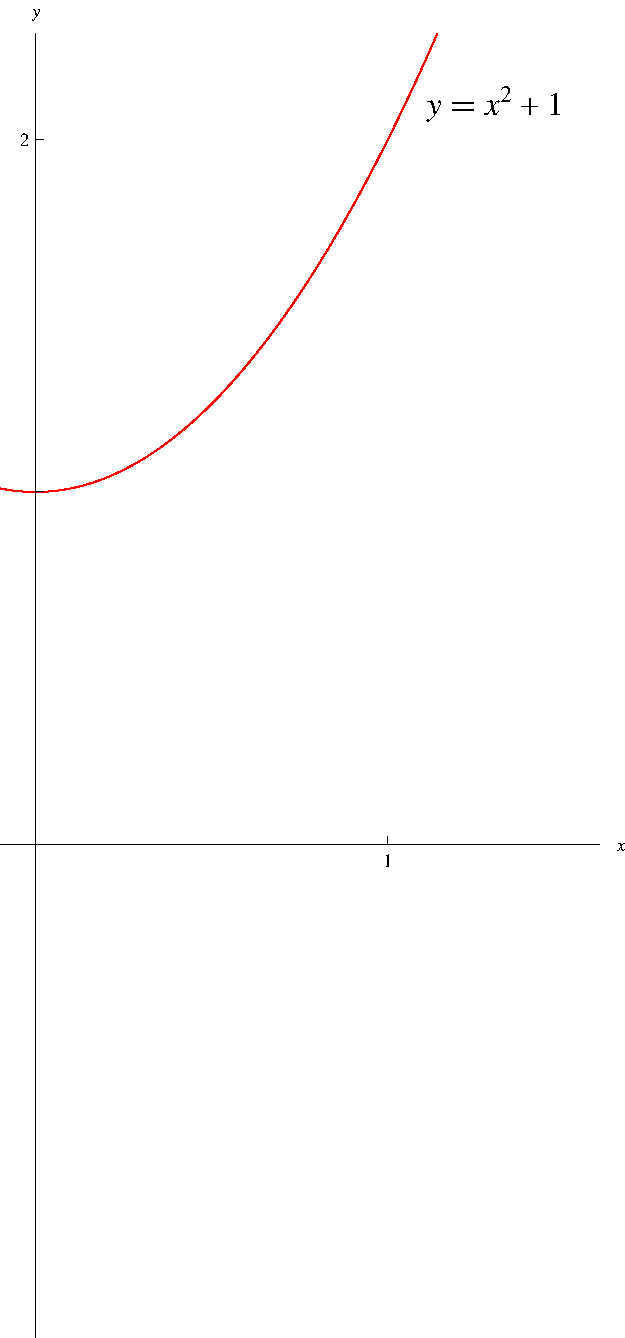
\includegraphics[height=3.3cm]{volumes/pictures/06-02-washerb.pdf} %
%}%
%\only<handout:0| 3>{%
%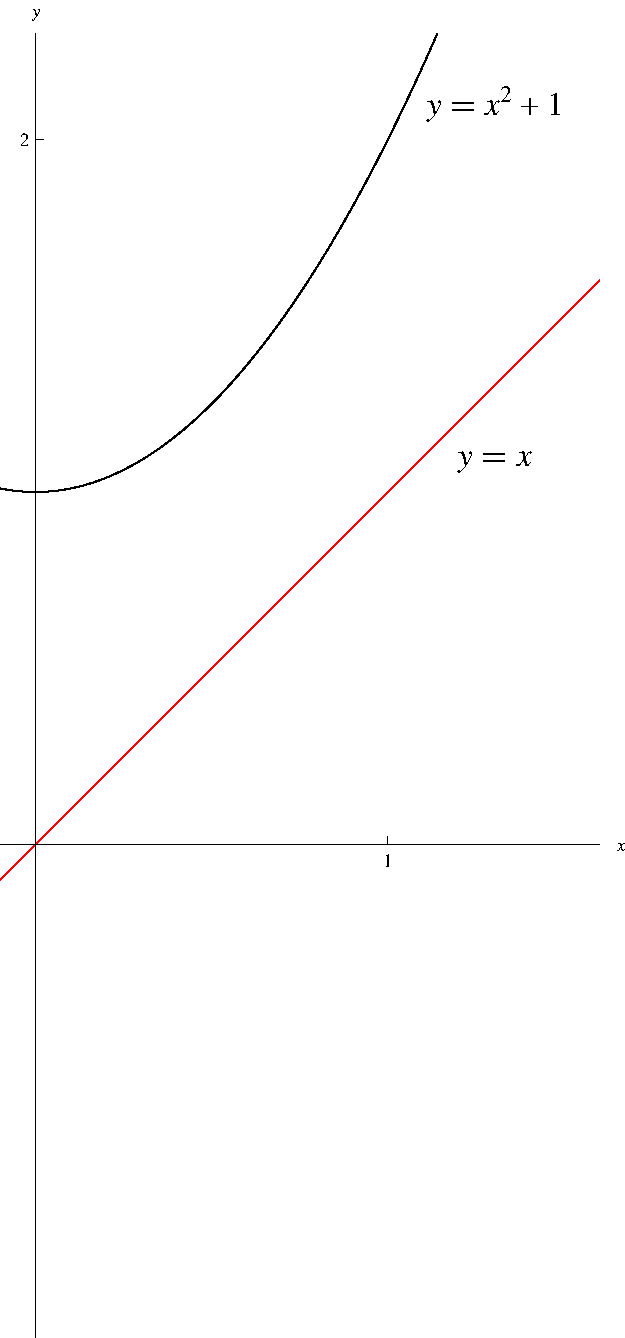
\includegraphics[height=3.3cm]{volumes/pictures/06-02-washerc.pdf} %
%}%
%\only<handout:0| 4>{%
%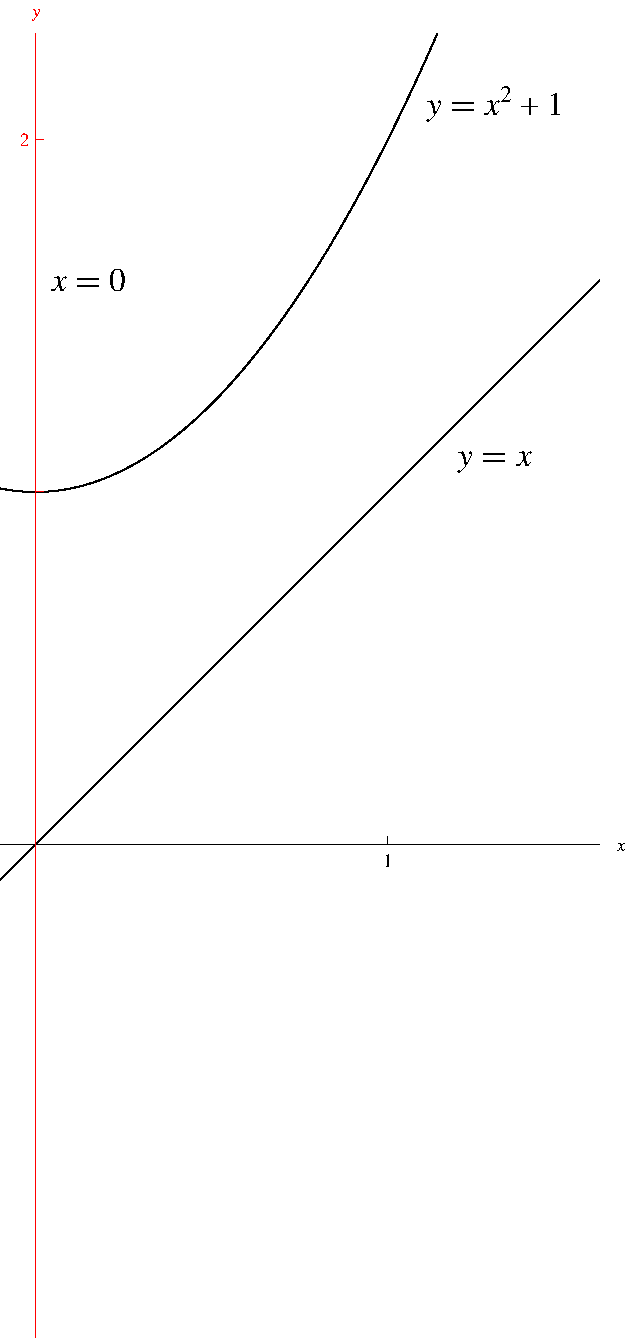
\includegraphics[height=3.3cm]{volumes/pictures/06-02-washerd.pdf} %
%}%
%\only<handout:0| 5>{%
%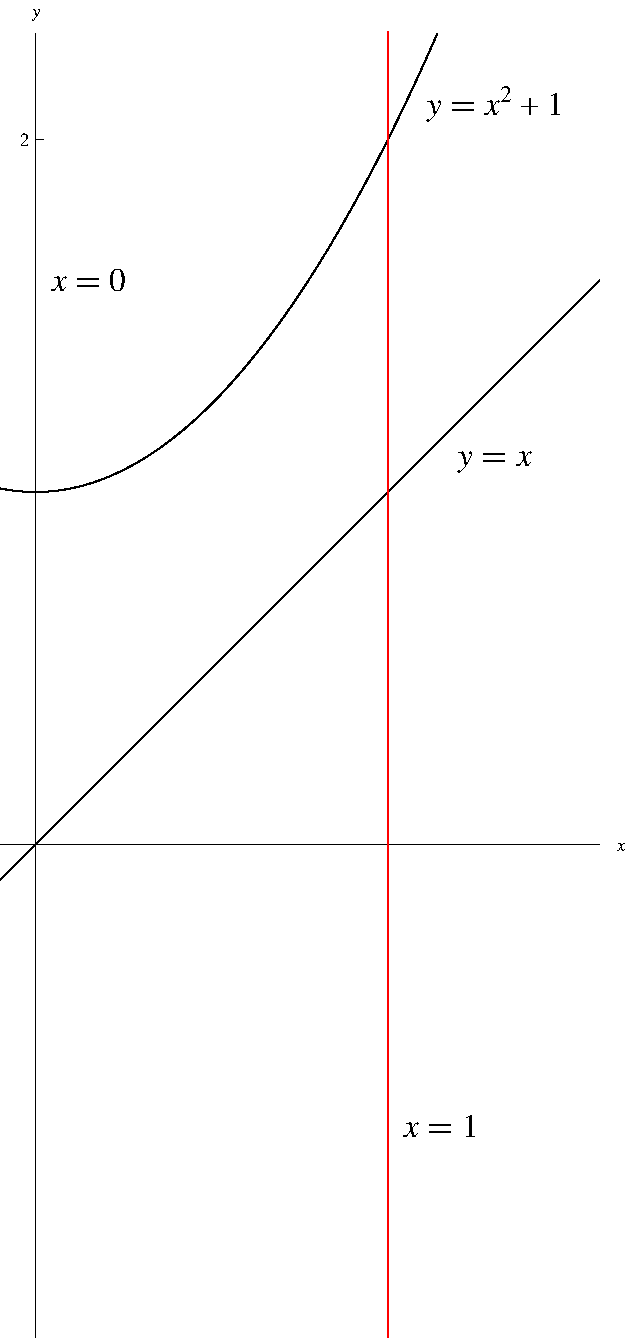
\includegraphics[height=3.3cm]{volumes/pictures/06-02-washere.pdf} %
%}%
%\only<handout:0| 6>{%
%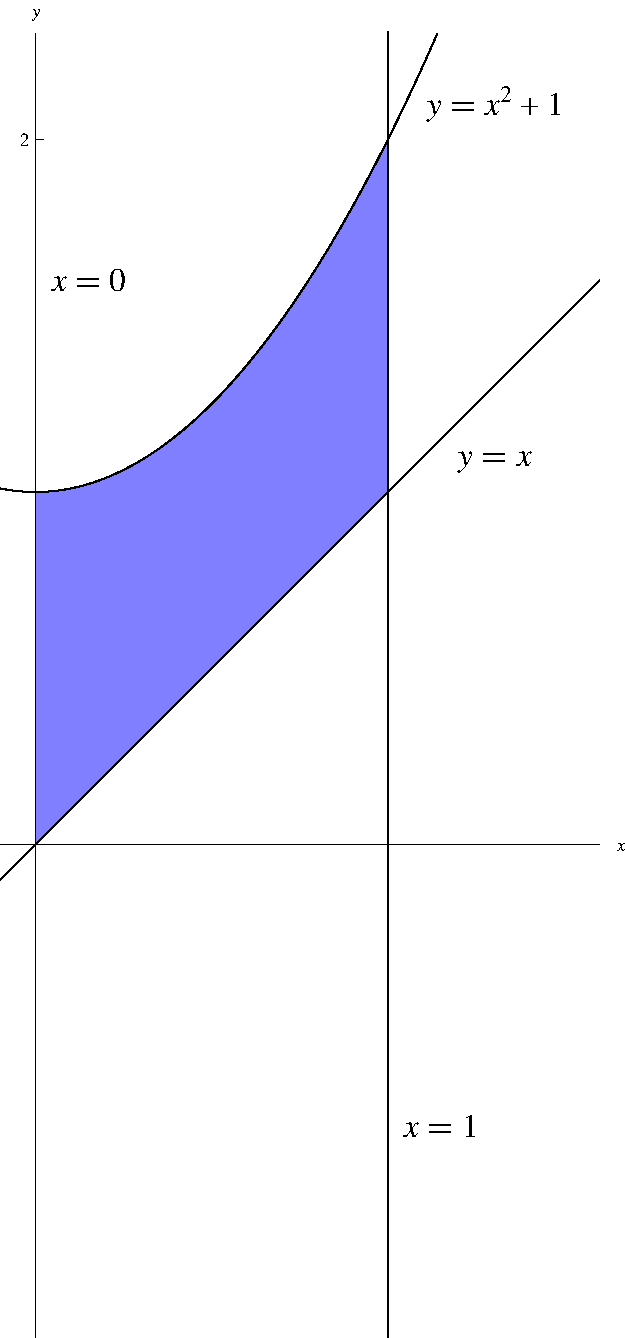
\includegraphics[height=3.3cm]{volumes/pictures/06-02-washerf.pdf} %
%}%
%\only<7->{%
%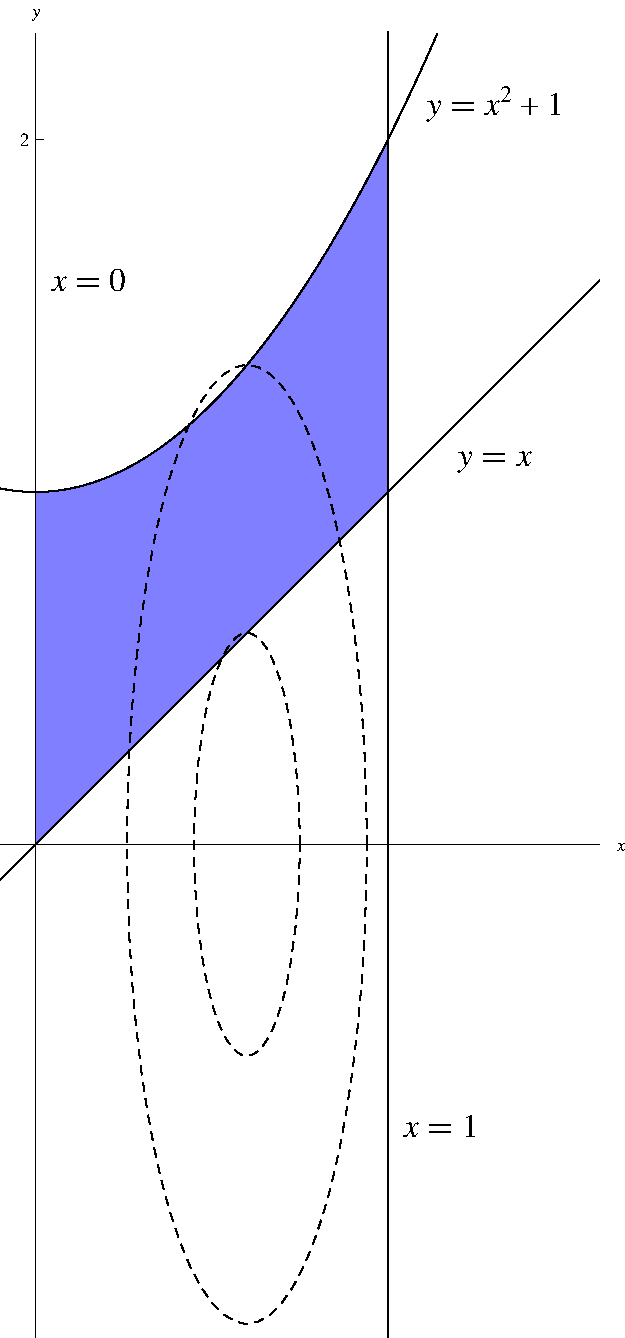
\includegraphics[height=3.3cm]{volumes/pictures/06-02-washerg.pdf} %
%}%

\column{.65\textwidth}
Find the volume of the solid obtained by rotating about the $x$-axis \alertNoH{ 6}{the region bounded by \alertNoH{ 2}{$y = x^2+1$}, \alertNoH{ 3}{$y = x$}, \alertNoH{ 4}{$x = 0$}, and \alertNoH{ 5}{$x = 1$}}.

\uncover<handout:2-|15->{%
\uncover<15->{Cross-section: }\uncover<16->{washer, center: $x-$axis.} 

\noindent\uncover<18->{%
\alertNoH{18}{\alertNoH{31}{Inner} radius, $ r $:} $\fcAnswer{19}{x,}$ 

\alertNoH{22,23}{\alertNoH{30}{Outer} radius, $ R $:} $\fcAnswer{23}{x^2+1},$ 
}%
}%uncover

\uncover<handout:3|1->{
$
\begin{array}{@{}r@{}c@{}l}
\uncover<26->{V & = & \displaystyle \int_{{\fcAnswer{28}{0} }}^{{\fcAnswer{28}{1}}} \alertNoH{29}{ \pi(R^2-r^2)} \diff x \\
&=& \uncover<29->{ \ds  \int_0^1 \left(\alertNoH{29}{ \alertNoH{30} {\alertNoH{32}{\pi} \alertNoH{33}{(x^2+1)^2}} - \alertNoH{31}{\alertNoH{32}{\pi} \alertNoH{33}{x^2} } } \right) \diff x}}\\%
\uncover<32->{ & = &\displaystyle %
\alertNoH{32}{\pi} {\alertNoH{34-38} {\int}}_{\!\!\!0}^1 \left( \alertNoH{33}{ \alertNoH{34-35}{x^4} + \alertNoH{36-37}{x^2} + \alertNoH{38,39}{1} } \right) \alertNoH{34-39}{  \diff x}%
}\\%
\uncover<34->{&  = &\displaystyle %
\pi {\left[ \fcAnswerUncover{34}{35}{\frac{x^5}{5}} + \fcAnswerUncover{34}{37}{\frac{x^3}{3}} + \fcAnswerUncover{34}{39}{x} \right]}_0^1%
}\\%
\uncover<40->{&  = &\displaystyle \pi \left( \frac{1}{5} + \frac{1}{3} + 1\right) \uncover<41->{= \frac{23}{15}\pi}}%
\end{array}
$
}
\end{columns}
\end{example}
\end{frame}
% end module volumes-washer
